\section{Пример II}

\subsection{Постановка задачи}
\renewcommand{\labelenumi}{\arabic{enumi})}
Задана ЗЛП в каноническом виде:
\begin{equation}
	F(\vec{X}) = 2x_1 - 5x_2 - x_3 + x_4 \to max,
\end{equation}

\begin{equation}
\begin{cases}
x_1 + 3x_2 - x_3 + x_4 = 1 \\
2x_1 + 3x_3 - x_4 = 2 \\
x_1, x_2, x_3, x_4 \ge 0
\end{cases}
\end{equation}.

Необходимо:
\begin{enumerate}
\item Решить исходную ЗЛП методом искусственного базиса;
\item Решить исходную ЗЛП графически;
\end{enumerate}

\subsection{Решение исходной ЗЛП методом искусственного базиса}
Введем искусственные переменные и приведем к каноническому виду.
Для нахождения максимума, умножим целевую функцию на -1.
Заметим, что вектор во втором столбце уже является
единичным после деления строки на 3.

$$-F(\vec{X}) = -(-2x_1+5x_2+x_3-x_4+Wx_5) \to max$$
\begin{equation}
\label{cannonical}
\begin{cases}
\frac{1}{3} x_1+x_2 - \frac{1}{3} x_3 + \frac{1}{3} x_4=\frac{1}{3} \\
2x_1+3x_3-x_4+ s_5=2\\
x_i, s_i \ge 0 \\
\end{cases}
\end{equation}

\begin{center}
\begin{tabular*}{\textwidth}{@{\extracolsep{\fill}}|c|c|c|c|c|c|c|c|c|c|}
\hline
$i$ & Базис & $C_i$ & B & $C_1 = -2$ & $C_2 = 5$ & $C_3 = 1$ & $C_4 = -1$ & $C_5 = W$ & $\Theta_i$ \\
\hline
$1$ & $P_2$ & $5$ & $0,3333$ & $0,3333$ & $1$ & $-0,3333$ & $0,3333$ & $0$ & --\\
$2$ & $P_5$ & W & $2$ & $2$ & $0$ & $3$ & $-1$ & $1$ & $0,6667$\\
\hline
$m+1$ & ~ & ~ & $1,667$ & $3,667$ & $0$ & $-2,667$ & $2,667$ & $0$ & ~ \\
\hline
$m+2$ & ~ & ~ & $2W$ & $2W$ & $0W$ & $3W$ & $-1W$ & $0W$ & ~ \\
\hline
\end{tabular*}
\end{center}
\begin{center}
\begin{tabular*}{\textwidth}{@{\extracolsep{\fill}}|c|c|c|c|c|c|c|c|c|c|}
\hline
$i$ & Базис & $C_i$ & B & $C_1 = -2$ & $C_2 = 5$ & $C_3 = 1$ & $C_4 = -1$ & $C_5 = W$ & $\Theta_i$ \\
\hline
$1$ & $P_2$ & $5$ & $0,5556$ & $0,5556$ & $1$ & $0$ & $0,2222$ & $0,1111$ & $1$\\
$2$ & $P_3$ & $1$ & $0,6667$ & $0,6667$ & $0$ & $1$ & $-0,3333$ & $0,3333$ & $1$\\
\hline
$m+1$ & ~ & ~ & $3,444$ & $5,444$ & $0$ & $0$ & $1,778$ & $0,8889$ & ~ \\
\hline
$m+2$ & ~ & ~ & $0W$ & $0W$ & $0W$ & $0W$ & $0W$ & $-1W$ & ~ \\
\hline
\end{tabular*}
\end{center}
\begin{center}
\begin{tabular*}{\textwidth}{@{\extracolsep{\fill}}|c|c|c|c|c|c|c|c|c|c|}
\hline
$i$ & Базис & $C_i$ & B & $C_1 = -2$ & $C_2 = 5$ & $C_3 = 1$ & $C_4 = -1$ & $C_5 = W$ & $\Theta_i$ \\
\hline
$1$ & $P_1$ & $-2$ & $1$ & $1$ & $1,8$ & $0$ & $0,4$ & $0,2$ & $1$\\
$2$ & $P_3$ & $1$ & $0$ & $0$ & $-1,2$ & $1$ & $-0,6$ & $0,2$ & $1$\\
\hline
$m+1$ & ~ & ~ & $-2$ & $0$ & $-9,8$ & $0$ & $-0,4$ & $-0,2$ & ~ \\
\hline
$m+2$ & ~ & ~ & $0W$ & $0W$ & $0W$ & $0W$ & $0W$ & $-1W$ & ~ \\
\hline
\end{tabular*}
\end{center}
Получен оптимальный план: $X^{опт} = (1;0;0;0;0)$,
и оптимальное значение целевой функции $F^{опт} = 2$.

\subsection{Решение исходной ЗЛП графическим методом}
\begin{figure}[ht]
\centering
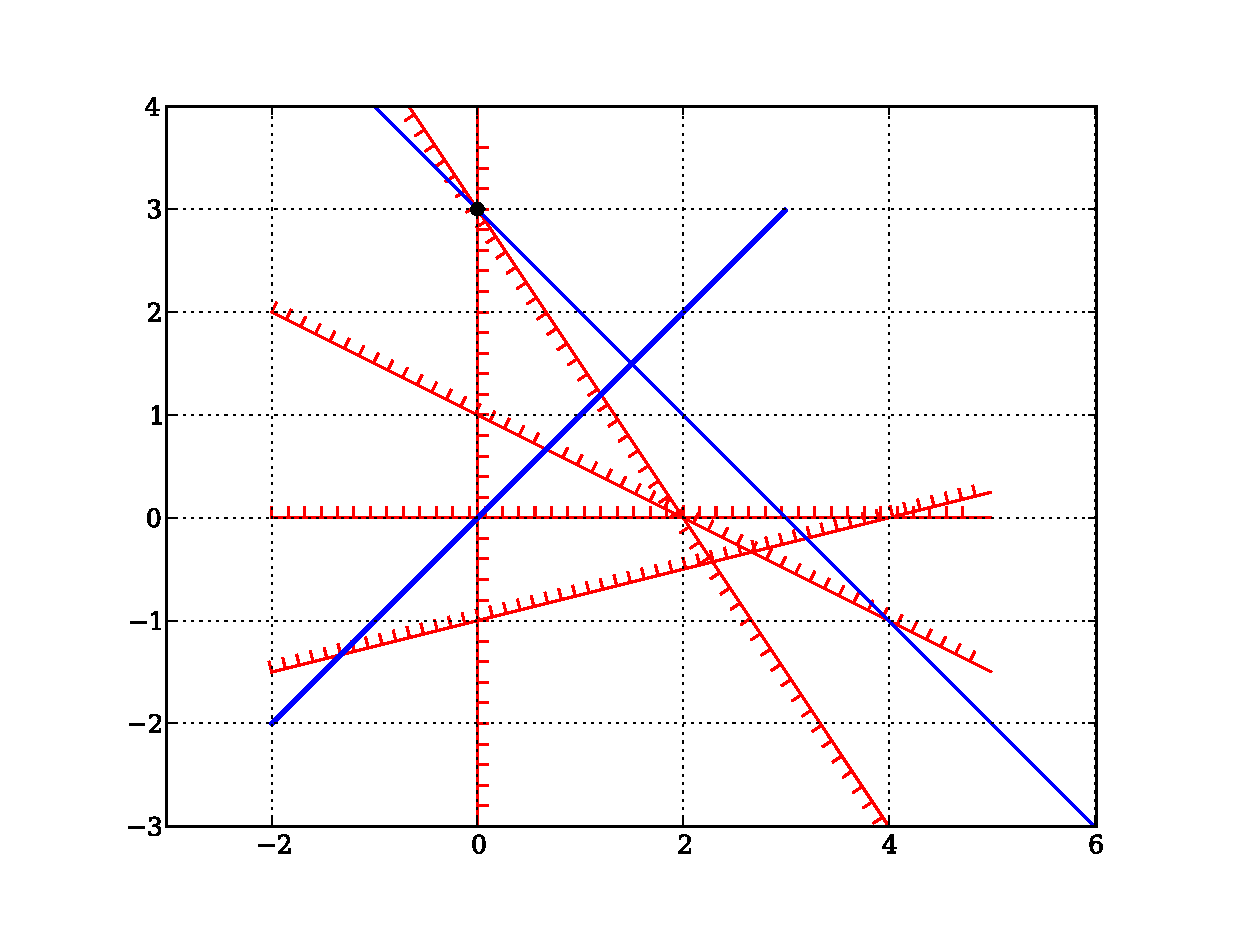
\includegraphics[width=\textwidth]{img/21}
\caption{Решение графическим методом}\label{21}
\end{figure}